\documentclass[tikz,convert={outfile=.svg}]{standalone}
 \usepackage{tkz-euclide}
\newcommand{\cercle}[4]{
\node[circle,inner sep=0,minimum size={2*#2}](a) at (#1) {};
\draw (a.#3) arc (#3:{#3+#4}:#2);
}

\begin{document}
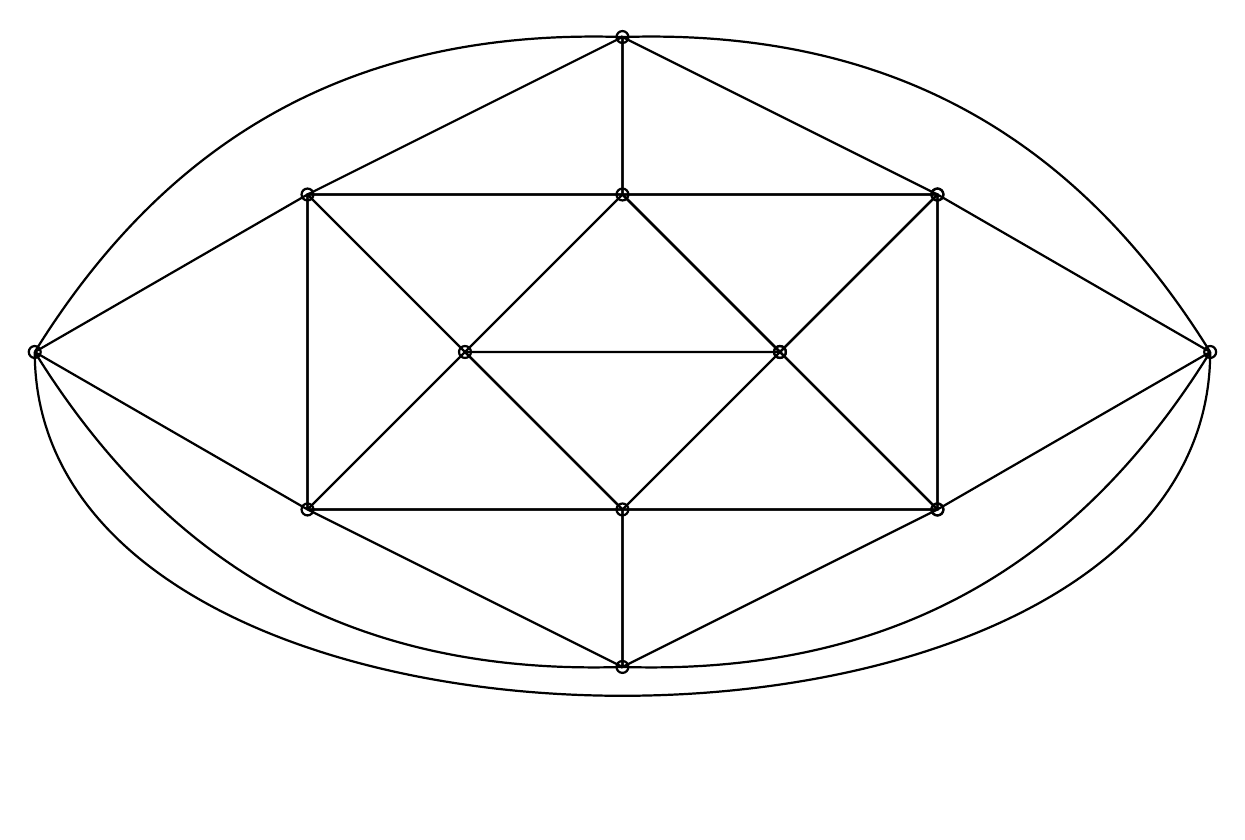
\begin{tikzpicture} 
[
    thick
]
\draw (0,0) circle (.5ex) -- (8,0) -- (8,4) -- (0,4) -- (0,0);
\draw (0,0) -- (2,2) -- (4,0) circle (.5ex);
\draw (0,4) circle (.5ex) -- (2,2) -- (4,4);
\draw (4,4) circle (.5ex) -- (6,2) -- (2,2);
\draw (2,2) circle (.5ex)-- (4,0) -- (6,2) circle (.5ex);
\draw (4,4) -- (6,2) -- (8,0);
\draw (8,0) circle (.5ex) -- (6,2) -- (8,4);
\draw (8,4) circle (.5ex) -- (6,2) circle (.5ex) -- (4,4);

\draw (0,0) -- (4,0) -- (4,-2) circle (.5ex) -- (0,0);
\draw (4,0) -- (8,0) circle (.5ex) -- (4,-2) -- (4,0);

\draw (0,4) -- (4,4) -- (4,6) circle (.5ex) -- (0,4);
\draw (4,4) -- (4,6) -- (8,4) circle (.5ex) -- (4,4);

\draw (0,0) -- (-sqrt{12},2) circle (.5ex) -- (0,4) -- (0,0);
\draw (8,0) -- (8+sqrt{12},2)  circle (.5ex) -- (8,4) -- (8,0);

\draw (4,-2) to[bend left] (-sqrt{12},2);
\draw (-sqrt{12},2) to[bend left] (4,6);
\draw (4,6) to[bend left] (8+sqrt{12},2);
\draw (8+sqrt{12},2) to[bend left] (4,-2);
\draw (-sqrt{12},2) to[bend right = 90] (8+sqrt{12},2);
 

\end{tikzpicture}
\end{document}